\subsection{Introduction}

The electronics of the Camera Assembly consist of two main parts. First is the Control and Communication Board and second is the Mainboard with Analog Front-End (AFE), Detector, Power Supply and Driver Modules. 
Principal parts and functions of the boards and modules are presented within the block diagram of \ref{fig:cam_overview}. 

\begin{figure}[H]
\centering

\includegraphics[width=\textwidth]{pict/cam_overview.png}
\caption{NEOSTEL camera block diagram}
\label{fig:cam_overview}
\end{figure}

The processing platform of the Control and Communication Board is based on a Xilinx Zynq System-on-Chip (SoC) solution that includes a two-core Cortex A9+ application processor and one Field-Programmable Gate Array (FPGA). It also contains a number of integrated peripheral interfaces like Ethernet, SPI, I2C, CAN, USB etc. as well as two DDR3 memory controllers. 
The system runs both Linux and RTOS operating systems in an AMP scenario, with Linux being responsible for the high level control and maintenance and with RTOS being in charge of time critical tasks. The entire communication is based on the Ethernet interface. A PTP synchronization protocol provides a microsecond synchronization capability. A serial port is used as standard console output for diagnostic purposes.
The Mainboard integrates controllers for the analogue front-end, CCD sensor (detector) TEC module, diagnostics and sensors.
The system is controlled via EPICS and provides server functionality. Image data will be double buffered and sent to a remote facility server in FITS format.

\subsubsection {Electronic System Features}
\begin{itemize}
\item Low noise 16MP CCD sensor readout – images are handled in a self-describing FITS format with additional diagnostic information
\item Shutter control with accurate start/stop position feedback implemented in the FPGA in the external shutter module
\item Environment measurements (humidity, temperature, position)
\item EPICS SCADA support with EPICS server implementation for system diagnostics and control
\item High speed interface: 1 Gbps Full Duplex Ethernet through SFP transceivers with full hardware PTP support including time-stamping
\item Internal and external trigger
\item Time synchronization via PTP
\item Heterogeneous system with both RTOS (for time-critical procedures) and Linux (for interfacing flexibility and easy data processing with low latency control and a diagnostics path)
\item Universal CCD data readout with flexible FPGA logic and modular AFE
\item Innovative Xilinx Zynq SOC design with dual core Cortex A9+ and FPGA on one silicon DIE with shared subsystems.
\end{itemize}

\subsection{Camera modules location within camera}
Camera modules location within camera is presented in figure x.x in mechanical description of camera.

\subsection{Control and Communication Board}

A Communication Board block diagram is presented in figure \ref{fig:commbrd}.

\begin{figure}[H]
\centering
\includegraphics[width=\textwidth]{pict/commbrd_block.png}
\caption{Communication board block diagram}
\label{fig:commbrd}
\end{figure}

The Communication Board connects with the Mainboard. It is an interface between camera electronics and an external server. The role of this board is:
\begin{itemize}
\item The generation of timing signals for the CCD sensor
\item The generation of timing signals for the Analog Front-End module
\item The data collection from analog-to-digital converters and sensors
\item The communication via Ethernet
\item The time synchronization using a PTP protocol.
\end{itemize}

The main processing unit is a Zynq SoC, containing a two core ARM Cortex A9+ processor and the FPGA logic. This part supervises all onboard peripherals and CCD sensor operations. It also sets the proper voltage to supply and bias the CCD, drives the CCD signals, receives data from A/D converters and sends data via the Ethernet. The Zynq processor has been chosen due to its ability to support 1 or 10 Gbit Ethernet. 

The Zynq SoC uses two types of the memory. The first one is volatile (RAM) memory; the second one is non-volatile (FLASH) memory. The RAM memory keeps the data and is required for image processing purposes, whereas the FLASH memory contains the Linux file system. There is an additional storage device on the module - a Micro SD card is used to store system logs.

The Ethernet connection is established by a SFP/SFP+ transceiver. Thus a copper or optical Ethernet connection can be implemented. The internal power supply consists of two quad channel high efficiency DC/DC converters that supply all devices on the module. A detailed electrical scheme is presented in the mainboard file.
\todo[inline, caption={Datapath}]{Co to jest mainboard file}
\subsubsection{ZYNQ SOC}
The ZYNQ SoC manufactured by Xilinx is the most important part of the communication module. The XC7Z030-2FFG676I chip was chosen because of the four high speed transceivers implemented in the 676-ball BGA package.
It has two so-called high-range (HR) banks, three high-performance (HP) banks, processing system (PS) banks and a single high-speed GTX transceiver bank. HR, HP and GTX banks belong to the FPGA of the SoC. The PS banks belong to the processor part of the SoC.
Pins from HR banks drive UART, SPI, IIC, LVDS and MLVDS interfaces. There are also general-purpose pins to drive LEDs and to check the state of the push-button switches.
HP banks are used as an interface to the SDRAM DDR3 memory and as a LVDS interface.
PS banks are the ARM processor external interface. They are connected to the SDRAM DDR3, NAND Flash, NOR Flash and SD card. Some of the pins are general-purpose pins and drive LEDs and interfaces like IIC, SPI, CAN and UART. The ARM processor can boot from all non-volatile memories mentioned above. 
A general block diagram of the ZYNQ 7000 SoC is shown in figure \ref{fig:zynq} (Source: www.xilinx.com).

\begin{figure}[H]
\centering
\includegraphics[width=0.7\textwidth]{pict/zynq.png}
\caption{ZYNQ SOC block diagram}
\label{fig:zynq}
\end{figure}

\subsubsection{Clock generators}

There are five oscillators on the Communication Board \ref{tab:clocks}. Two of them are ARM system clocks; the other three drive GTX interfaces.

\begin{table}[]
\centering
\caption{Clock generators}
\label{tab:clocks}
\begin{tabular}{|l|l|l|l|}
\hline
Oscillator part number & Frequency & Connected to & Role \\ \hline
SiT8103AC-32-18E-33.33300X & 33,33 MHZ & ARM & System clock \\ \hline
570BBC000121DG & 10-280 MHz & ARM & RAM clock \\ \hline
ASFLMPLV-156.250MHZ-LR-T & 156,25 MHZ & FPGA & 10 Gbit Ethernet clock \\ \hline
LF VCXO026156 & 20 MHz & FPGA & White Rabbit clock \\ \hline
VM53S3-25.000-2.5/-30+75 with CDCM61004RHBT & 125 MHz & FPGA & White Rabbit clock \\ \hline
\end{tabular}
\end{table}

\subsubsection{VOLATILE MEMORY}
The Communication Board contains two banks of SDRAM DDR3 memory. Each bank contains two 16-bit 128Mx16 chips. The first memory group is controlled by the FPGA, the second by the ARM processor. The single memory chip has a capacity of 2Gb (512 MB). 

\subsubsection{NON-VOLATILE MEMORY}
There are three types of non-volatile memory on the Communication Board. The first one is a NAND Flash, ONFI compatible. The MT29F8G08ABBCAH4 memory was chosen. It is a single chip, 8Gbit (1GB), 8-bit NAND memory, to store the Linux file system.
The operating system data can also be stored into a NOR Flash. Two S25FL128SAGMFIR01 chips are used. A single one is a 128Mbit (16MB) Flash memory chip with a fast quad-SPI interface. 
The third memory is a micro SD card (user defined capacity). The TXS02612RTWR level translator is placed between the SoC and the SD card.
The Zynq Soc can boot from all of these memories. Boot-mode can be selected by using jumpers.
\todo[inline, caption={Datapath}]{Ten akapit w kilku miejscach jest mało logiczny}

\subsubsection{SEARAY CONNECTOR}
Searay connector (SEAF-20-01-X-10-X-RA) connects with the Mainboard. It delivers supplies and MLVDS and LVCMOS interfaces to the rest of the electronic circuitry.

\subsubsection{MINI-SAS CONNECTOR}
A Mini-SAS connector is optional and can be used in the future. It is electrically connected to the Zynq GTX transceivers. Thus PCIe x4 or 40Gbit Ethernet can be implemented.
\subsubsection{USB}
A user-friendly debugging interface is implemented. There are two CP2102-GM USB-to-UART bridges connected to the FPGA part of the SoC.
The detailed electrical schematic is presented in the USB.SchDoc-file.

\subsubsection{SFP+}
One GTX transmitter and one receiver of the SoC are connected to the SFP+ module. This has been chosen such due to the ability to transceiver fast 1 and 10 Gbit signals used in Ethernet connections. The resistor tree provides backward compatibility with the SFP module.
The detailed electrical scheme is presented in the SFP+.SCHDoc-file.

\subsubsection{RS485 AND OPTO-INTERFACE}
These interfaces are used for trigger and shutter control. The RS485 is bi-directional; the opto-interface has four inputs.

\subsubsection{Power supply}
The power supply chain of the Communication Board is presented in the block diagram of figure \ref{fig:powersup}.

\begin{figure}[H]
\centering
\includegraphics[width=\textwidth]{pict/power_supply.png}
\caption{Power supply chain of the Communication Board}
\label{fig:powersup}
\end{figure}


P12V0 is the main power supply from the external power adaptor. There are two quad synchronous buck converters that convert the main supply into several voltages. Each converter channel consists of a common controller/driver (XRP7724) and of external high-power transistors (STL60N32N3LL). P1V2, P1V6, P2V9, and P5V0 rails supply the mainboard through a Searay Connector. Other voltages from a second DC/DC converter, P1V0, P1V5, P1V8, and P3V3 supply the SoC, some peripherals, and LDOs. LDOs are used to supply noise-sensitive parts e.g. SoC GTX transceivers or the DDR3 reference voltage. 
Detailed electrical schemata are presented in the Power.SchDoc-, Power supply linear.SchDoc- and Power supply switching.SchDoc-files. 
Shutter interface and trigger signals will be delivered using standard Amphenol, M12 ruggedized connectors.
The layout of the Communication Board is presented in Figure 5 39.

\begin{figure}[H]
\centering
\includegraphics[width=\textwidth]{pict/commbrd_layout.jpg}
\caption{Layout of the communication board}
\label{fig:commbrd_layout}
\end{figure}

\subsubsection{LAN interface and data link transfer aspects}
A SFP+ cage (Small Form-factor Pluggable Transceiver) provides the communication interface of the camera. Several types of optical or copper transceivers will be installed. Gigabit Ethernet or even PCI Express Gen II protocols can be used without hardware modifications.
To enable the communication between several cameras, Gigabit Ethernet and a TCP protocol are implemented. This provides for each camera the option of a fully autonomy control and data acquisition. Since each camera has an independent operating system, the measurement data (FITS files) can be stored directly using NFS or FTP protocols on suitable servers.
The main system architecture data path starts at the CCD sensor readout (16 ADCs) and ends at the FPGA fabric on the Zynq SoC. The Data can be read from the sensor and sent to the processing system in real time. The latter packages the data into FITS format and sends the according FITS files to the control system (PC server) via a Gigabit Ethernet interface (Figure 5 40). Gigabit Ethernet is implemented by means of a GTX transceiver and PCS/PMA logics. It cooperates with a hardcoded MAC block that is directly connected to the ZynQ CPU subsection.
The AFE produces 16 serial streams of 100Mbit/s each. These streams are de-serialized by the IP Core and transferred by the AXI stream to the ZynQ memory.

\begin{figure}[H]
\centering
\includegraphics[width=\textwidth]{pict/datapath.png}
\caption{Datapath}
\label{fig:datapath}
\end{figure}

\todo[inline, caption={Datapath}]{Poprawić, bo rysunek ma błędy}

\subsection{Main Board}

\begin{figure}[H]
\centering
\includegraphics[width=\textwidth]{pict/mainbrd.png}
\caption{Main Board block diagram}
\label{fig:mainbrd}
\end{figure}

Figure \ref{fig:mainbrd} provides the block diagram of the systems connected to the Mainboard. Analog Device ADC (AD7960) 18bit SAR converters have been selected due to their low noise abilities, high SNR, and relative high sampling rate. Four ADCs will be implemented to sample each CCD channel – the goal is to oversample the signal and to utilize a digital signal processing to filter white and correlated noise. To lower the jitter of the sampling clocks, an additional buffer will be used that distributes the signal point-to-point.
The Analog-Front-End (AFE) board contains a circuitry designed to process raw analogue data from the CCD matrix. Depending on its implementation it can be CDS or adaptive filtering and buffering of the input signal. Several implementations are considered and the one with best noise characteristics will be chosen for the final version of the camera.
The Shutter driver is enclosed in the shutter case and implemented as a linear amplifier with a current limiter (through feedback), working in a half bridge configuration. The position detection of the shutter blades is provided by dedicated sensor. It is connected with the Mainboard using a sealed connector where RS485, I2C, and logic control signals are distributed.
The Mainboard also contains the Peltier Thermoelectric Cooler (TEC) with a half bridge driver set trough a PWM controller. An additional feedback circuit is used on the board to measure the current of the Peltier module. The PWM operation is synchronized with the CCD operation to prevent noise interference propagation to the AFE chain.
The board also has a dedicated ADC for reading the PT-1000 temperature sensors that measure the temperature in different parts of the camera. 

\subsubsection{CCD and CCD driving signals}
The main task of the camera Mainboard is to provide power to all other modules of the camera - generated from one single standard 24V power entry and the CCD control.  All voltages needed by the detector module - power, bias, reset and clocking upper and lower levels - are adjustable by Digital-to-Analog Converters (DACs). The programmable range fits within the safety region defined by the sensor manufacturer.
The sensor is critical part of the design. Therefore, the NEOSTEL camera was designed to support at least two different CCD vendors – E2V and Andanta, given the possibility that one CCD prototype could not be available at the time of deployment. A third vendor, Fairchild Imaging does not produce suitable sensors anymore. Table \ref{tab:CCD} summarizes the parameters of three foreseen sensors.
The E2V sensor is described by the manufacturer in a substrate biased configuration at positive level (instead of ground) to enable positive voltage biasing and clocking. However, a bipolar operation was selected, with the substrate connected to the ground to preserve similar supply and driving circuits for both sensors. The resulting bias voltages corrected all driving and biasing voltages specified by the manufacturer. Thanks to this approach, similar voltage levels can drive both sensors and differences can be compensated by means of resistive dividers at LDO regulators. \\
When it comes to the CCD sensor decision, E2V CCD231-84 is considered as a better solution while Andanta CCD4150A is the backup one. CCD231-84 provides a better dark current noise characteristic, which is one of the key parameters for the camera. An additional advantage over the alternative sensor is that it has additional inputs that allow for a faster binning and cleanup process.

\begin{savenotes}
\begin{table}[!htbp]
\centering
\caption{CCD comparison}
\label{tab:CCD}
\begin{tabular}{|c|c|c|c|c|}
\hline
 & CCD4150A & CCD230-84 & CCD231-84 & Units \\ \hline
Manufacturer & Andanta & E2V & E2V & \\ \hline
Operation mode & NIMO/MPP & MPP & NIMO & \\ \hline
Resolution &4096 x 4096 & 4096 x 4096  & 4096 x 4096 & pix \\ \hline
Pixel size & 15 x 15 & 15 x 15  & 15 x 15 & $\mu$m \\ \hline
Image Area &61.44 x 61.44& 61.44 x 61.44 & 61.44 & mm \\ \hline
Illumination & Backside & Backside & Backside &  \\ \hline
Clocking sequence & three--phase& four--phase & four--phase &  \\ \hline
Outputs &4& 4 &4 &  \\ \hline
Fill factor &near 100& near 100 &  near 100 & \% \\ \hline
Maximum rate of heating or cooling & N/A & 5 & 5 & K/min \\ \hline
Dark current & 5.0 $\frac{e^{-}\cdot h}{pix}$ (163K) &2.0 $\frac{e^{-}\cdot s}{pix}$ (248K)&  0.2 $\frac{e^{-}\cdot s}{pix}$ (153K) & \\ \hline
Image FWC (NIMO/MPP)  & 300k/150k &  NA/150k & 350k/NA  & $e^{-}$ \\ \hline
Output FWC (OG mode)  & TBD  & 450k/900k & 200k/600k & $e^{-}$ \\ \hline
Output amplifier sensitivity & 5 & 2.5 & 7 & $\mu V/e^{-}$ \\ \hline
Output rms noise  & 2.5 (@100kHz)  & 4 (@50kHz) & 2 (@50kHz) & $ e^{-}$ \\ \hline
Charge transfer efficiency & >99.999 &  >99.999 &  >99.999 & \% \\ \hline
Spectral range & 300--1060 & 300--1060 & 300--1060 & \% \\ \hline
Minimum full frame read time & & 1.064 & 1.531 & s\\ \hline
Minimum full frame dump time &  & 0.256 & 0.179 & s\\ \hline
ROI (512x512 pix) read time \footnote{Details described in section \ref{sec:windowing}} & & 0.377 & 0.360 & s\\ \hline
\end{tabular}
\end{table}
\end{savenotes}

The CCD sensor requires several bias voltages that are generated by low noise – Low Drop Out (LDO) regulators that are trimmed by DACs.
The CCD drivers require a low ripple and stable power supply. Therefore, all needed power voltages are provided by LM1117/LM337 LDO and linear regulators that are trimmed by DACs. The industrial temperature range for all semiconductors was chosen.
For the horizontal and vertical transfer electrodes, EL7457 drivers are used. At the output of these drivers, resistors are installed that limit dv/dt. A too high dv/dt would cause charge efficiency degradations. \\
Control signals for CCD drivers as well as AFE are generated by Pattern Generator \ref{sec:patgen} IP-core within FPGA on Communication Board. 16 ADCs are dedicated for readout of the CCD data. \\

\subsection{Hardware monitoring sensors}
All of camera PCBs are equipped with various sensors including temperature, humidity, voltage sensors, accelerometer and tachometer. Function of the accelerometer is to detect vibrations caused by e.g. the shutter. Some sensors located in critical parts of the camera have capability of hardware monitoring and power shutdown. \\
List of sensors used in the camera is presented below:

\begin{description}

\item \textbf{Communication board} \hfill \\
\begin{itemize}
\item voltages
\item humidity
\item 2x temperature
\end{itemize}

\item \textbf{Mainboard} \hfill \\
\begin{itemize}
\item humidity
\item temperature
\item 3x temperature
\item acceleration (3-axis)
\item coolant volumetric flow rate - tachometer
\end{itemize}

\item \textbf{CCD board} \hfill \\
\begin{itemize}
\item humidity
\item temperature
\end{itemize}

\item \textbf{Shutter} \hfill \\
\begin{itemize}
\item humidity
\item temperature
\end{itemize}

\end{description}

\subsection{Shutter electronic design}

\subsubsection{Introduction}

The Electronics of the shutter is placed inside the shutter’s replaceable module. It contain an FPGA that controls the shutter mechanism and receives the information of the shutter position from the position sensors.

Figure \ref{fig:shutconn} shows the connection between camera and shutter modules. The shutter can also be controlled via RS485 or analog trigger signals. The trigger signals (ACTION) for each shutter module are opto-isolated and available on the back panel of the camera. Output signals (CONFIRM) are asserted when correct shutter opening or closing occurs.
The I2C bus is used only to upload an FPGA firmware directly from camera. It is connected to flash memory from which the FPGA download it's firmware.

\begin{figure}[H]
\centering
\includegraphics[width=1\textwidth]{pict/shutter_connection.png}
\caption{Shutter-camera connection block diagram}
\label{fig:shutconn}
\end{figure}

Shutter electronic module contains: motor driver, two blade position sensors, temperature and humidity sensor and accelerometer. Figure \ref{fig:shutblk} presents the block diagram of the shutter’s module internals. 

\begin{figure}[H]
\centering
\includegraphics[width=1\textwidth]{pict/shut_block.png}
\caption{Shutter's module block diagram}
\label{fig:shutblk}
\end{figure}

\subsubsection{Position sensor}

For the precise knowledge about the exact position of the shutter blade(s) during opening and closing, a high precision encoders signals is recorded and timestamped. Shutter is equipped with 2 position sensors, one absolute and one incremental.

The absolute shutter positioning system is based on a capacitance measurement. Sensor have two capacitors that are made of PCBs with copper plate. Capacity of those capacitors (C1 and C2 on \ref{fig:shutsens}) is changing during movement of the blade: one increase his capacity and the other decreases it (and the other way during movement in the opposite direction). One can change the differential capacity to the coroleted voltage output, so it is possible to plot the voltage vs blade position characteristic. Detailed description of sensor design is in 5.1.6.3 subsection.

To translate a capacity to voltage a high frequency generator is connected to capacitors – leading to output's DC component linearly depends on the capacity. This signal is filter to get only DC component, then it is amplified to get the best dynamic range and then it is measure by ADC. \ref{fig:shutsens}.

\begin{figure}[H]
\centering
\includegraphics[width=0.9\textwidth]{pict/shut_sens.png}
\caption{Shutter's capacity position sensor schematic}
\label{fig:shutsens}
\end{figure}

Second position sensor is the incremental magnetic sensors RLS RLC2IC. Sensor has 3 differential lines as an output 'A','B' and 'Z'. 'A' and 'B' signals creates the incremental quadrature pair that give a pulse after every 5um of displacement. Quadrature encoding give a possibility to detect the direction of the moment. 'Z' signal give reference pulse each 2mm \ref{fig:shut_mag_sens_wave}. These signals are feed to differential line receiver (DS26LV32AT) to change signal to LVCMOS level to be compliant with FPGA inputs \ref{fig:shut_mag_sens_sch}.

\begin{figure}[H]
\centering
\includegraphics[width=0.7\textwidth]{pict/shut_sens_magnetic.png}
\caption{Shutter's magnetic position sensor schematic}
\label{fig:shut_mag_sens_sch}
\end{figure}

\begin{figure}[H]
\centering
\includegraphics[width=0.7\textwidth]{pict/shut_sens_magnetic_waveform.png}
\caption{Shutter's magnetic position sensor waveform}
\label{fig:shut_mag_sens_wave}
\end{figure}

\subsubsection{Driver}
Each shutter motor has an independent driver, allowing controlling the movement of each blade. The separation of the individual channels allows a synchronization of the speed of both blades despite the differences in the direction of the gravitational force. The diagram below shows one single shutter driver channel.

\begin{figure}[H]
\centering
\includegraphics[width=0.7\textwidth]{pict/shut_drv.png}
\caption{Shutter driver (actuator)}
\label{fig:shutdrv}
\end{figure}

A single SPI Digital to Analogue Converter (DAC) with two independent analogue outputs (DAC7612) controls the shutter driver channel. To provide the motors with sufficient current, an additional differential buffer is used. This buffer is implemented on OPA548 operational amplifiers with an output current up to 5A. The buffers have an implemented thermal shutdown to protect the shutter driver from overheating. Buffers are connected to output headers by LC PI-type filters to minimize the EMI.
The positive output of the differential buffer is connected to a current monitor, which is implemented as a 10MOhm resistor with an AD8031 operational amplifier, set to a gain of 20. The output of the current monitor is connected to an ADS7945 SPI SAR 14-bit ADC and creates a feedback path. This solution allows implementing control algorithms that can modulate the DAC output to accomplish a constant current drive instead of a constant voltage.
Two modes of shutter driver operation are being considered – an operation with feedback from the shutter positioning subsystem or an operation based on lookup tables. In the first solution, a digital controller e.g. PID is feed with the shutter position and the motor drive current. This allows the adjustment of the speed of the blade. In the second solution, a table of drive values is created, based on calculations and adjusted by experiments. The table will contain a set of analogue values for the DACs that will be applied within a specific time interval to obtain a repeatable shutter movement.
\subsubsection{Sensors}

Each shutter module is equipt with addition sensors:
\begin{itemize}
\item Temperature and Humidity (HDC1000) - detecting the overheat of the shutter's electronic and measuring the humidity around the camera window to predict the window heater work.
\item Accelerometer (ADXL343) - measure vibration generated by shutter
\end{itemize}

\subsubsection{Control}
%\todo[inline, caption={Failsafe shuttera}]{ Schemat nie uwzględnia co robimy w przypadku %błędu, żadnego failsafe/override dla procedury. To jest mechanika, jeśli error to %zostawiamy shutter wiszący w połowie? W jaki sposób jest przewidywana sygnalizacja stanów %i w jaki sposób jest przewidywana obsługa otoczenia shuttera w każdym z nich? /PZi}

Each Shutter module interface contains:

\begin{itemize}
\item Action line (input) - triggering opening or closing of the blade
\item Confirm line (output) - confirmation of opening or closing of the blade
\item RS485 bus (slave) - communication between camera and shutter module
\end{itemize}

RACZJE USUNAC TEN OBRAZEK NIŻEJ
\begin{figure}[H]
\centering
\includegraphics[width=0.7\textwidth]{pict_ipc/shutter_control.png}
\caption{Shutter internal control state chart}
\label{fig:shutctrl}
\end{figure}

For system point-of-view shutter control description refer to section \ref{sec:shutctrl}.

\paragraph{Shutter control signals waveforms}

The motion of the blade is triggered by rising edge of the ACTION line. The ACTION line has to by 'HIGH' for at least 10us for shutter to trigger the event, this is to ensure that debouncing mechanism don't discard the pulse as a glitch. 
When event occurs, shutter starts moving the blade and recording motion data. When the movement of the blade is finished the CONFIRM line change to 'high', which is a signal to the camera that shutter opening or closing is 
completed. The ACTION line toggle the current shutter state, so the normal operation during taking picture is to pulse the ACTION line to open the shutter, then after the exposure time pulse it again to close the shutter blades.

Each shutter module has it own ACTION and CONFIRM line, the RS485 bus is in multi-drop configuration with camera as a master and two shutter module as a slaves. The CONFIRM line is used to ensure that each shutter blade did it action correctly. The CONFIRM line 
stay 'high' until the shutter module received a reset command via RS485. The ACTION line don't trigger any action before the shutter is not reset. During the reset, all the capture motion data are erase, so the normal operation will be to first read those data, then reset the shutter. The waveform diagram below shows the typical shutter operation during image acquisition.

\begin{figure}[H]
\centering
\includegraphics[width=1\textwidth]{pict/Sht_Wafeform.png}
\caption{Shutter interface waveform for opening and closing}
\label{fig:shtwf}
\end{figure}

During the movement the motion data are analysed and the errors are detected.
Below is a shutter module state diagram.

\begin{figure}[H]
\centering
\includegraphics[width=0.7\textwidth]{pict_ipc/Sht_FSM.png}
\caption{Shutter stage diagram}
\label{fig:shtfsm}
\end{figure}

From shutter point of view, there is no difference between external (diagnostic mode) and internal control.

\paragraph{Communication protocol} 
%\\newline
Shutter communicate with the camera via RS485 interface. Camera is a master and two shutter modules are slaves that only can respond to command, they can't start the transmission. CRC is used as an error-detecting method, if the error is detected the receiver send a error code and data frame is retransmitted.


Each data frame sent from camera to shutter contains:
\begin{itemize}
\item Start frame (1 byte)
\item Slave adress  (1 byte)
\item Command code (1 byte)
\item Data bytes (optional - depends on command)
\item CRC bytes  (2 byte)
\item Frame end byte (1 byte)
\end{itemize}

Each data frame sent from shutter to camera contains:
\begin{itemize}
\item Frame start byte (1 byte)
\item Data bytes (depends on command)
\item CRC bytes (2 byte)
\item Frame end byte (1 byte)
\end{itemize}

	\begin{table}[H]
\begin{center}
    \begin{tabular}{| l || l  || l  |}
    \hline
    \bf{Command}				& \bf{Code (hex)} & \bf{Respond}\\ \hline
	Reset						& 0  		 	  & ACK / NACK	\\ \hline
	Send motion data			& 11  		 	  & data 		\\ \hline
	Send temperature			& 12  		 	  & data		\\ \hline
	Send humidity				& 13  		 	  & data		\\ \hline
	Send acceleration			& 14  		 	  & data		\\ \hline
	Send coil current			& 15  		 	  & data		\\ \hline
	Send absolute position		& 16  		 	  & data		\\ \hline
	Send incremental position	& 17  		 	  & data		\\ \hline
	Error						& 2  		 	  & Error code	\\ \hline
	Open shutter				& 31  		 	  & ACK / NACK	\\ \hline
	Close shutter				& 32  		 	  & ACK / NACK	\\ \hline
	Move to position			& 33  		 	  & ACK / NACK	\\ \hline
	Send status					& 4  		 	  & Status code	\\ \hline
	Shutter emergency shutdown 	& 5  		 	  & -			\\ \hline
	Retransmission request 		& 6  		 	  & depend		\\ \hline
    \end{tabular}
    \end{center}
    \caption{Shutter command list}
	\label{table:shut_err_table}
\end{table}

	\begin{table}[H]
\begin{center}
    \begin{tabular}{ | l || l  |}
    \hline
    \bf{ACK/NACK}		& \bf{Code} 	\\ \hline
	Acknowledge			& 0 	\\ \hline
	Non Acknowledge 	& 1 	\\ \hline
    \end{tabular}
    \end{center}
    \caption{Shutter acknowledge coding table}
	\label{table:shut_err_table}
\end{table}
	
	\begin{table}[H]
\begin{center}
    \begin{tabular}{ | l || l  |}
    \hline
    \bf{Error} 							& \bf{Code} 	\\ \hline
	No problem							& 0 	\\ \hline    
	Shutter mechanical problem			& 1 	\\ \hline
	Shutter overheat					& 2 	\\ \hline
	Shutter unknown error				& 3 	\\ \hline
    \end{tabular}
    \end{center}
    \caption{Shutter error coding table}
	\label{table:shut_err_table}
\end{table}

	\begin{table}[H]
\begin{center}
    \begin{tabular}{ | l || l  |}
    \hline
    \bf{Status}				& \bf{Code} 	\\ \hline
	Shutter open			& 0 	\\ \hline
	Shutter closed			& 1 	\\ \hline
	Shutter during motion	& 2 	\\ \hline
	Shutter motion finished & 3 	\\ \hline		
	Shutter fail 			& 4 	\\ \hline
    \end{tabular}
    \end{center}
    \caption{Shutter status coding table}
	\label{table:shut_err_table}
\end{table}

\subsection{CCD cooling subsystem}

\subsection{Camera time synchronization mechanism}
\subsubsection{Introduction}

The following actions of the camera are time-stamped:
\begin{itemize}
\item Trigger event
\item Start of shutter opening
\item Start of shutter closing
\item Start of CCD readout
\item Arming camera
\end{itemize}

The figure below \ref{fig:ptptopo} presents a scheme of the PTP synchronization subsystem. Each camera as well as processing server is connected to a common Gigabit Ethernet Switch with PTP capability. A PTP time master is used to distribute the time to the entire NEOSTEL installation.

%Dodane Pzi:
\todo[inline, caption={PTP - szerszy opis, doprecyzowanie}]{Opisac pobieżnie mechanizm synchronizacji PTP, również w przypadku używania w serwerach standardowych x86 - jest dobry dokument Fujitsu o tym - http://events.linuxfoundation.org/sites/events/files/slides/lcjp14\_ichikawa\_0.pdf jest to standard w przypadku rozproszonych tranzakcyjnych baz danych. W NEO, jeśli daemon PTP będzie działać to bierzemy wersję z HW TSTAMP i mamy wszystkie mechanizmy opisane w dokumencie (łącznie z phc), trzeba będzie na koniec sprawdzić implementację PTP pod kątem: działania na warstwie 2, warstwie 3, po TCP, UDP i IPv6.
PTP Time synchronization with the same algorithm will be used in every Neostel Camera server providing common time for all of the system./ PZi}

\begin{figure}[H]
\centering
\includegraphics[width=0.6\textwidth]{pict/ptp_topo.png}
\caption{PTP synchronisation network topology}
\label{fig:ptptopo}
\end{figure}

Utilizing NTP is also possible, using the standard Linux daemon service.
We are considering 2 possible PTP synchronisation solutions: one using built-in MAC and the other using dedicated PL IP core. Both solutions are described in detail below.

\subsubsection{Integrated MAC solution}

\begin{figure}[H]
\centering
\includegraphics[width=0.7\textwidth]{pict/soft_ptp.png}
\caption{PTP timestamping using integrated MAC PTP HW and Linux PTP driver}
\label{fig:softptp}
\end{figure}

The PTP synchronization schematic using built-in MAC is presented on figure \ref{fig:softptp}.
The ZynQ SoC Media Access Controller block is PTP-capable, including hardware packets timestamping. PTP synchronization is provided by dedicated Linux driver in cooperation with PTP-capable hardware in MAC. PTP time is kept in specialized, memory-mapped hardware register in MAC.  Microsecond synchronization accuracy is possible. \\
Camera event timestamping is implemented in software in each event's ISR. Each event triggers appropriate interrupt in CPU Core 1 (RTOS). Each event's ISR reads the time-stamp value from the PTP Ethernet register in MAC and assigns it to that specific event. Such solution is a compromise between complexity and accuracy, because the ZynQ does not provide direct hardware access to the time-stamp register in PTP MAC. Because interrupts are serviced on RTOS, both low jitter and delay are expected (sub-10 $\mu s$ range).